\documentclass{article}

\usepackage{graphicx}
\usepackage{natbib}
\begin{document}

A research group from Penn State has noticed strange behaviors with a quasar called 
J1011+5442.\cite{runnoe} After an observation in 2003, more recent observations in 
2013 and 2015 have revealed that the quasar's spectrum has changed significantly. 
This is behavior is highly unusual for a quasar, which is supposed to be a very 
bright, energetic blackhole accreting at the center of a galaxy. The quasar showed 
a 5100 $\AA$ monochromatic luminosity decrease of \textgreater 9.8 and broad 
$H\alpha$ luminosity decrease by a factor of 55 over a period of \textless 9.7 
years. 

\begin{figure}[h]
  \label{fig:plot}
  \caption{Spectrum of J1011+5442 in 2003 and 2015}
  \centering
  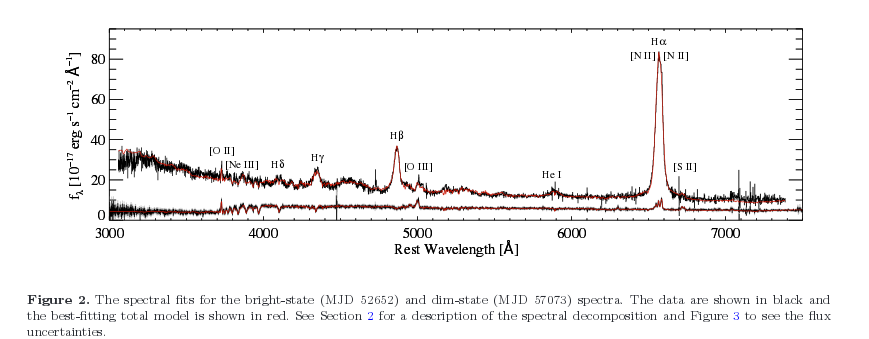
\includegraphics[scale=0.5]{fig2.png}
\end{figure}

The group proposes three possible mechanisms for these results. First, there 
could have been a large cloud that moved between Earth and the quasar that absorbed 
the high energy flux. This could be the case, as we see greatly reduced UV flux from 
the object in Figure 1. \ref{fig:plot} However, the calculated time required for a 
cold cloud to migrate that distance would be at least 30 years, which is far more 
than the 10 year timespan we observe. Second, it could be a large tidal disruption 
event during the first observation. This is also unlikely, as the luminosity spike 
lasted closer to six years instead of the average few-month timespan. Finally, and 
most likely, is we observed the 'turning off' of a quasar's AGN. If this is the 
case, it would be a very remarkable event that we observed. 

\bibliographystyle{plain}
\bibliography{ref}

\end{document}
